% Bagian Analisis Hasil Percobaan
\section*{Analisis Hasil Percobaan}
\indent
% Pada gambar \ref{fig:inirujukan} dapat dilihat bahwa pada tabel \ref{tab:labelini}

Pada praktikum ke-1 tentang Desain PCB menggunakan Fusion 360, kami membuat sebuah desain PCB dari rangkaian \textit{minimal system} ESP8266, rangkaian ini terdiri dari ESP8266, Connector UART, Connector Power, Regulator 3.3V (SOT223), 5 Resistor, 2 Kapasitor, dan 2 Switch. Rangkaian \textit{minimal system} dapat dilihat pada gambar \ref{fig:rawcircuit}.

\begin{figure}[htbp]
    \centering
    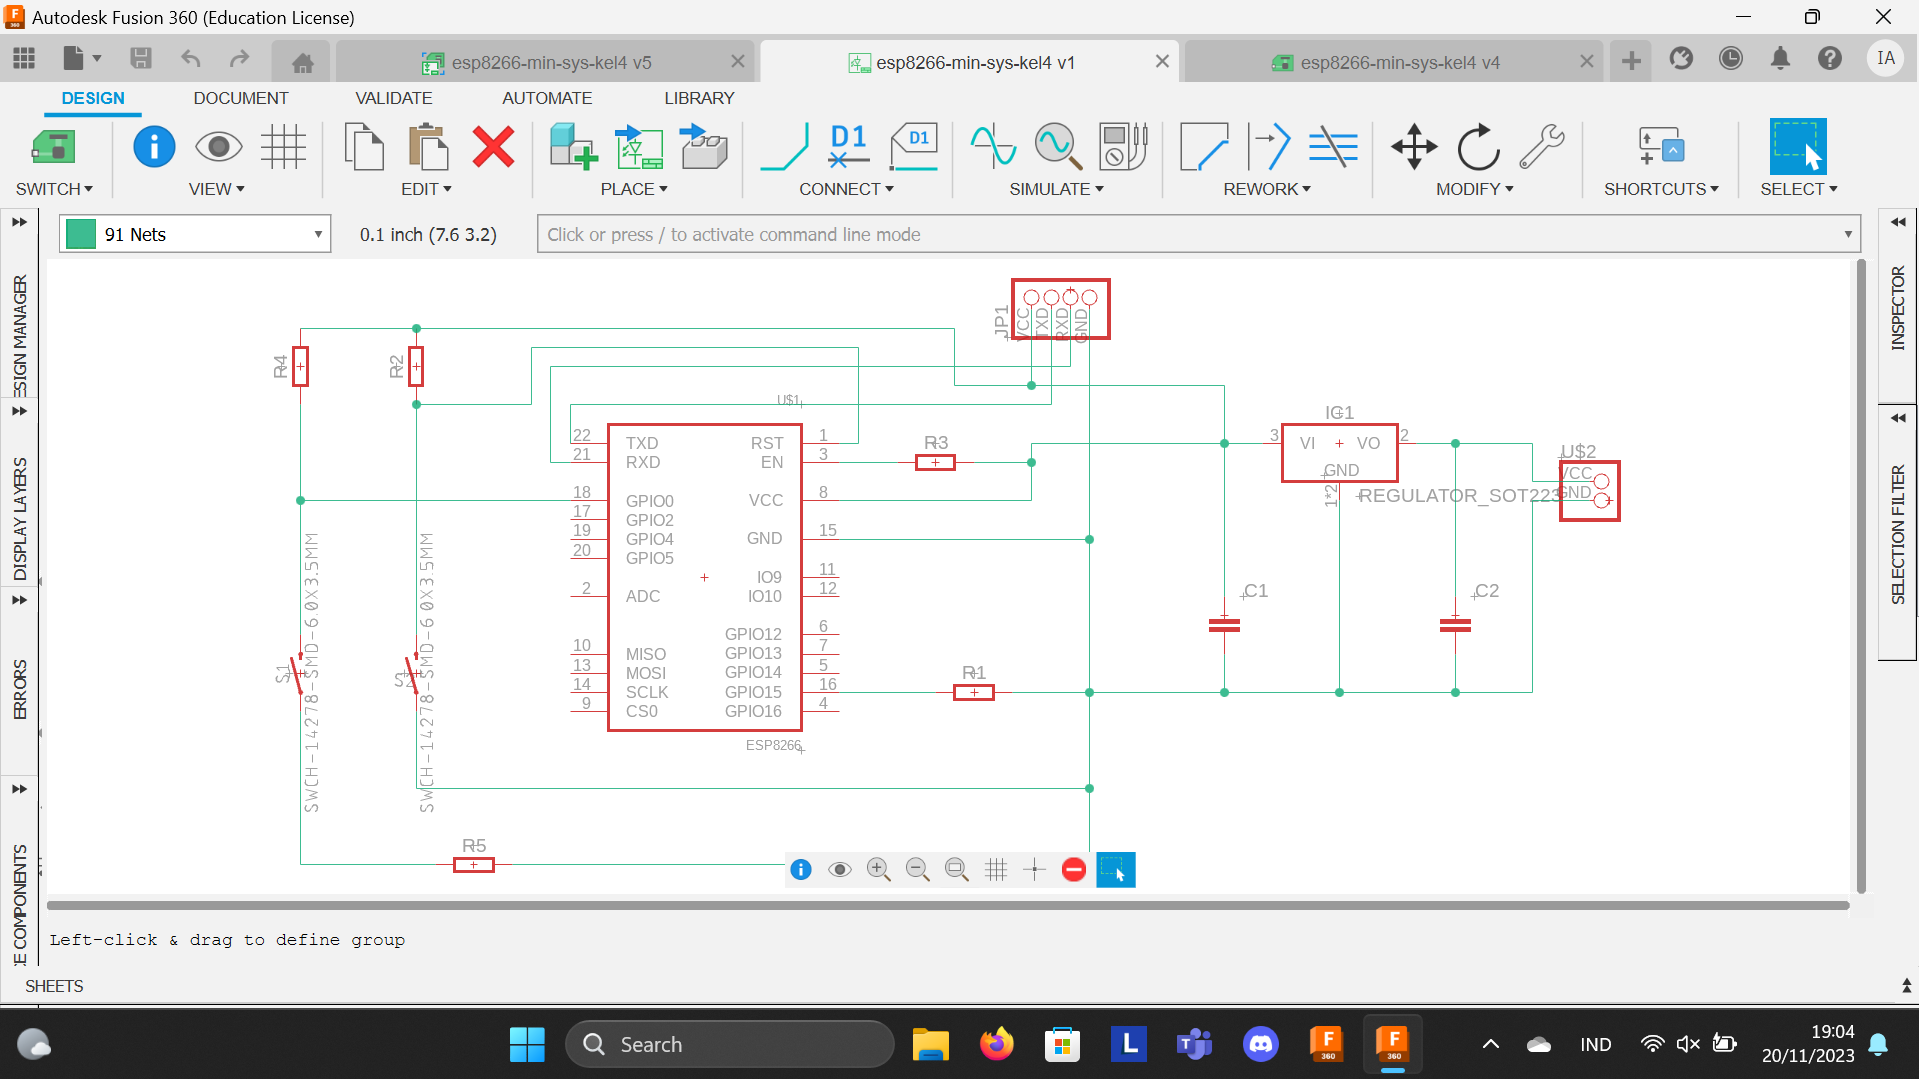
\includegraphics[width=0.4\textwidth]{img/raw-circuit.png}
    \caption{Desain Circuit \textit{Minimal System} ESP8266}
    \label{fig:rawcircuit}
\end{figure}

Setelah itu, kami mendesain layout PCB dari rangkaian \textit{minimal system} ESP8266 tersebut. Layout PCB dapat dilihat pada gambar \ref{fig:pcb-assembled}.

\begin{figure}[htbp]
    \centering
    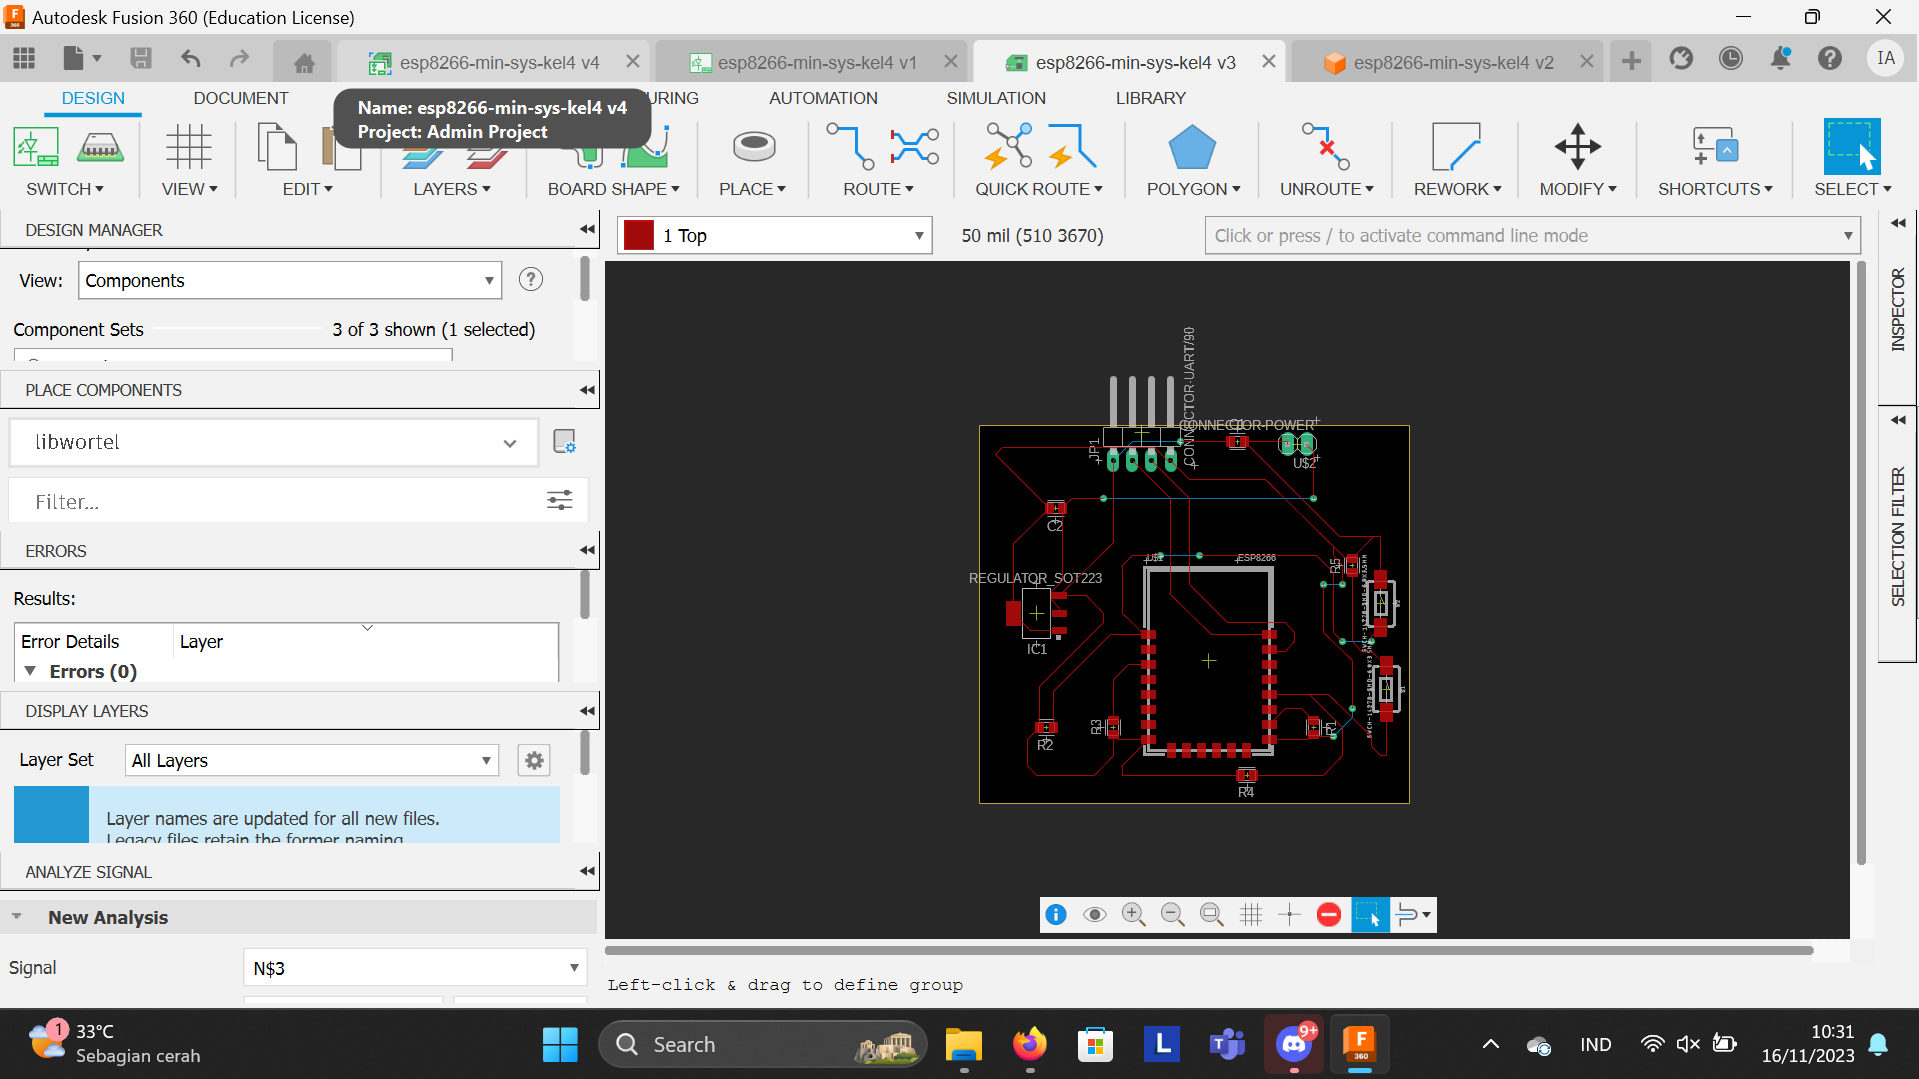
\includegraphics[width=0.4\textwidth]{img/pcb-assembled.png}
    \caption{Desain PCB yang telah dibuat \textit{layout}-nya}
    \label{fig:pcb-assembled}
\end{figure}

Setelah itu, kami men-\textit{generate} 3D model dari PCB yang telah dibuat. 3D model dapat dilihat pada gambar \ref{fig:3dmodel}.

\begin{figure}[htbp]
    \centering
    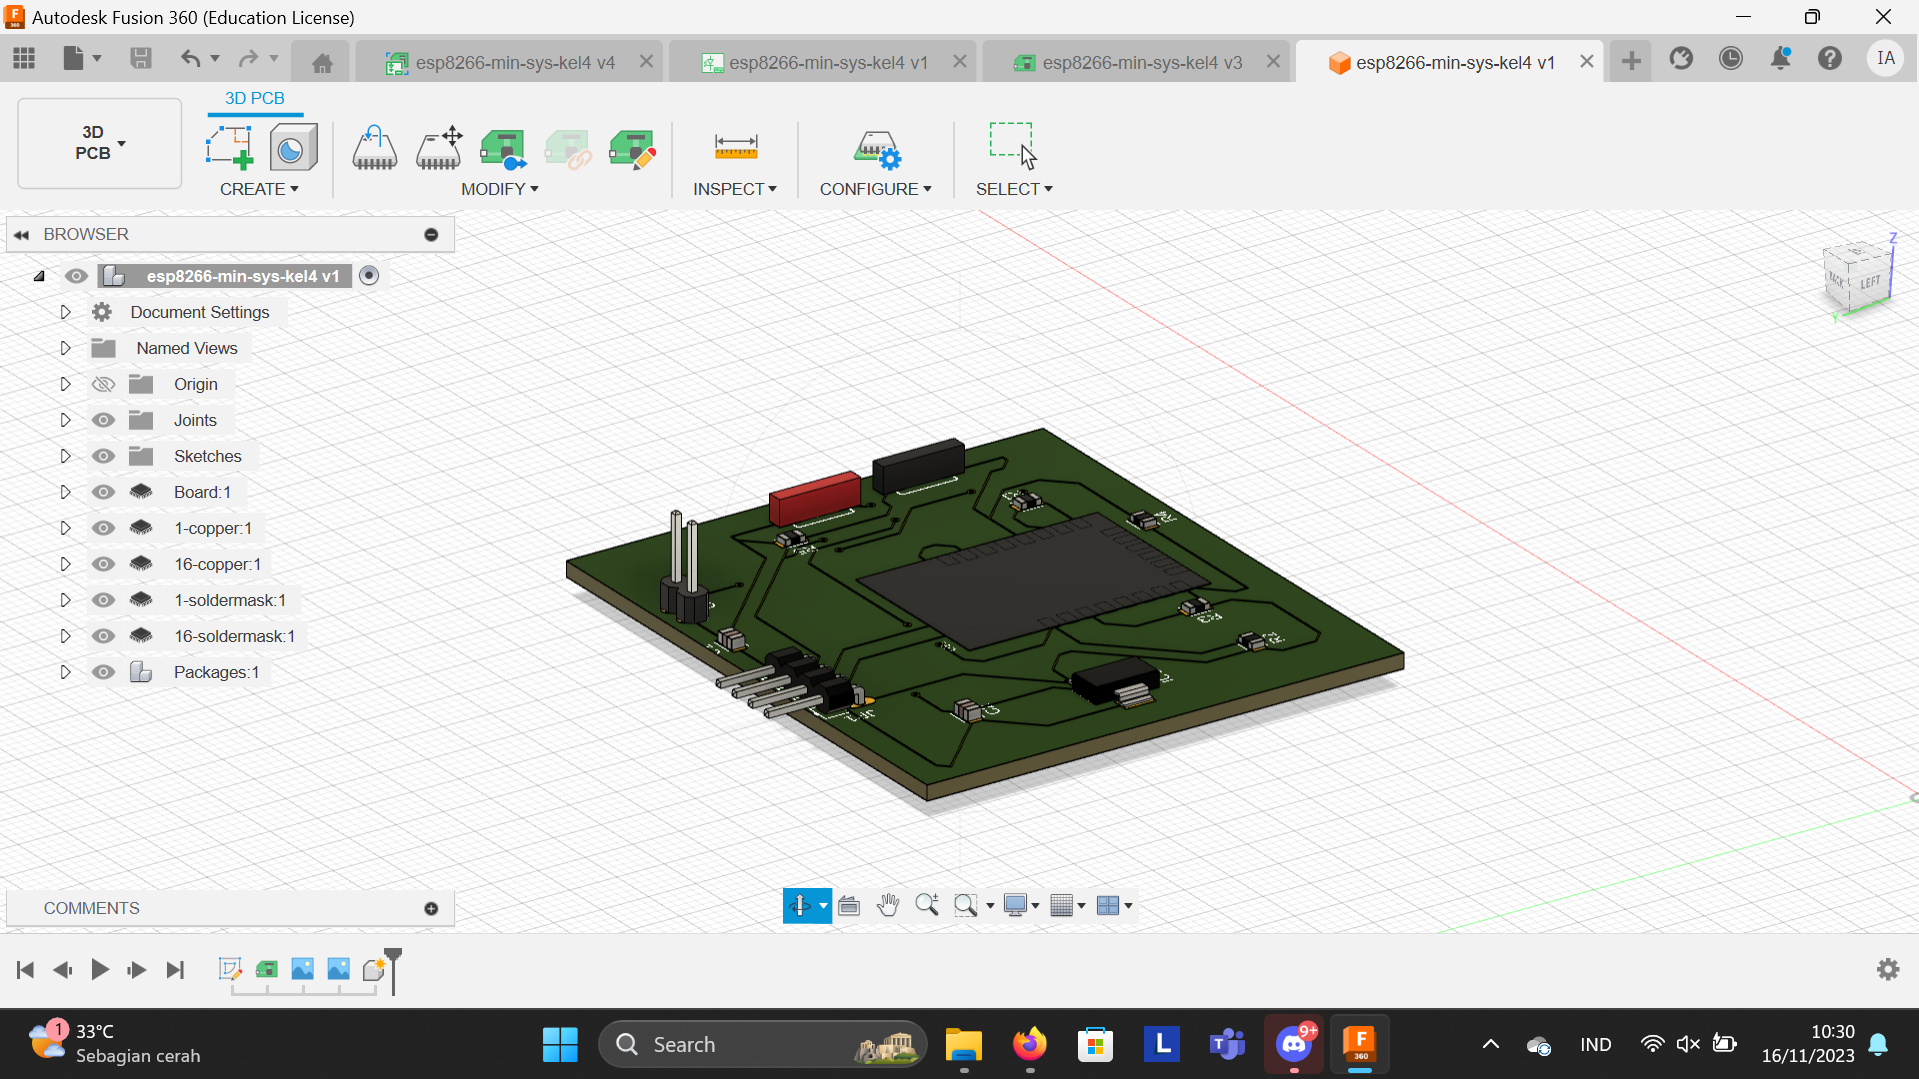
\includegraphics[width=0.4\textwidth]{img/fusion360.png}
    \caption{3D Model dari PCB yang telah dibuat}
    \label{fig:3dmodel}
\end{figure}

Praktikum secara teknis terdapat kendala kecil, seperti :

\begin{enumerate}
    \item Praktikan tidak menggunakan mouse, sehingga proses \textit{design} menjadi lebih lama.
    \item Device yang digunakan untuk praktikum tidak memiliki spesifikasi yang cukup untuk menjalankan Fusion 360, sehingga proses \textit{design} menjadi lebih lama.
\end{enumerate}

% \begin{table}[h]
%     \centering
%     \caption{Caption tabelnya}
%     \label{tab:labelini}
%     \begin{tabular}{|c|c|c|}
%     \hline
%     Kolom 1 & Kolom 2 & Kolom 3 \\
%     \hline
%     Data 1 & Data 2 & Data 3 \\
%     Data 4 & Data 5 & Data 6 \\
%     \hline
%     \end{tabular}
% \end{table}

\newpage